%!TEX root = ../thesis.tex
\chapter{Performance Analysis}
\label{chap:performance analysis}

\section{PnL}
According to Figure 6.1, after both backtesting and simulated trading, we have trading analyses that will be displayed on the web dashboard. Figure 7.2 shows the backtesting result. We can see that backtested from 2018 to 2019, we have a profit of over 1 million, which is about 25\% profit, starting with 1 million capital for each pair and 4 millions in total. All 4 pairs trades are profitable and the hit ratio is 100\%. The maximum drawdown is about only 3\%. The resulting Sharpe ratio is 2.5.

Cummulative PnL plot is also shown in Figure 6.2. Performance of our pairs trading model is much better than SP500 performance. The backtesting result shows that our trading model is very profitable, which is a contrast to our simulated trading result in Figure 6.4. There are several reasons that result in huge losses. First and the most important, our pairs trading model fails since pairs have different relationships during the first month of 2019 than the training data. SP500 index movement in 2018 is quite mean-reverting, where its constituents might also have stable relationships in this year. However, SP500 index at the start of 2019 is more momentum, where its constituents are likely to result in different relationships than in 2018. Second, we have flaws in our design of order book and order matching algorithm. Third, our trading model does not have stop loss. Further discussions of these issues and potential improvements are in conclusion.

\begin{figure}[h!]
\centering
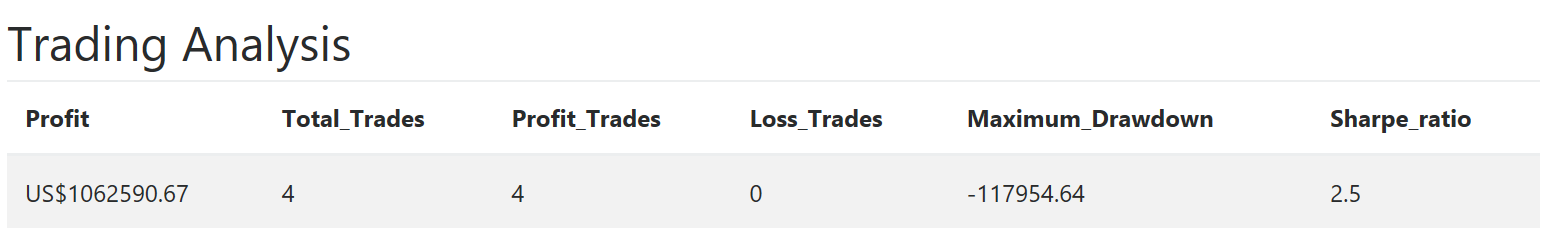
\includegraphics[scale=0.5]{performance_analysis/images/pnl1.png}
\caption{Backtesting Statistics}
\label{fig:backteststats}
\end{figure}

\begin{figure}
\centering
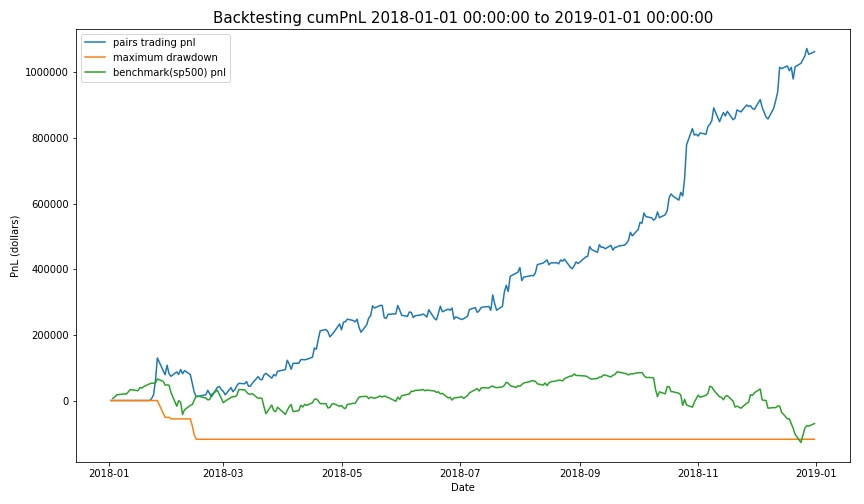
\includegraphics[scale=0.45]{performance_analysis/images/backtest_pnl.jpg}
\caption{Backtesting PnL}
\label{fig:backtest}
\end{figure}

\begin{figure}
\centering
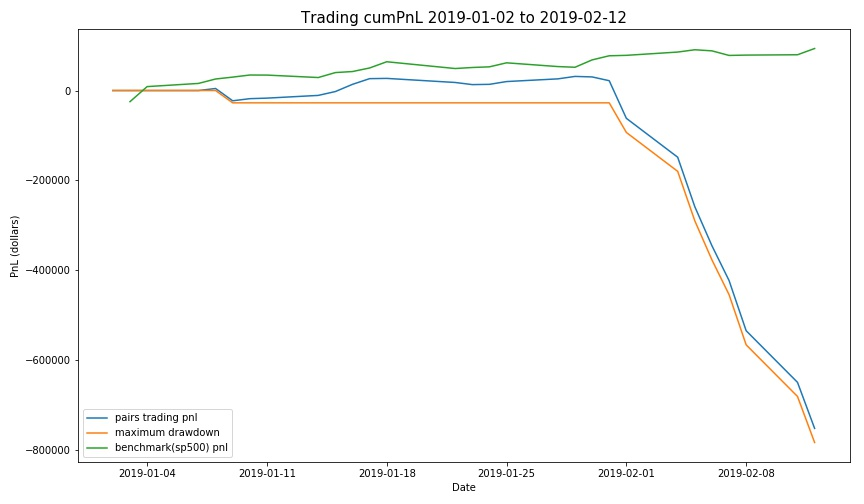
\includegraphics[scale=0.45]{performance_analysis/images/trade_pnl.jpg}
\caption{Simulated Trading PnL}
\label{fig:trading}
\end{figure}



\section{Web Dashboard}

Our web dashboard is built through flask. There are several modules on the web dashboard:
\begin{itemize}
    \item Home Page: displays our pairs trading strategy logic, shown in Figure 7.4;
    \item Stock Pairs: displays Table stockspairs;
    \item Building Model: displays Table pairprices;
    \item Back Testing: displays Table trades;
    \item Trading Analysis: displays performance analysis table and plotted PnL for backtesting result;
    \item Real Trading: displays performance analysis table and plotted PnL for simulated tradingg result;
\end{itemize}

Whenever a module button is clicked on the page, the program will run on the server/client side and the display will show when the process is finished. Each module has to run in order. For "Real Trading" module, it will wait for over 10 minutes until the performance result shows on the page. 

Flask will run on the main thread with the client side. We have another thread called client thread that will do simulated trading part with client/server communication. To do that, we need a global variable "bClientThreadStarted" to keep track if client thread start. It is set to false initially, and to true whenever simulated trading starts. The main thread will wait for client thread finishes to continue.

\begin{figure}
\centering
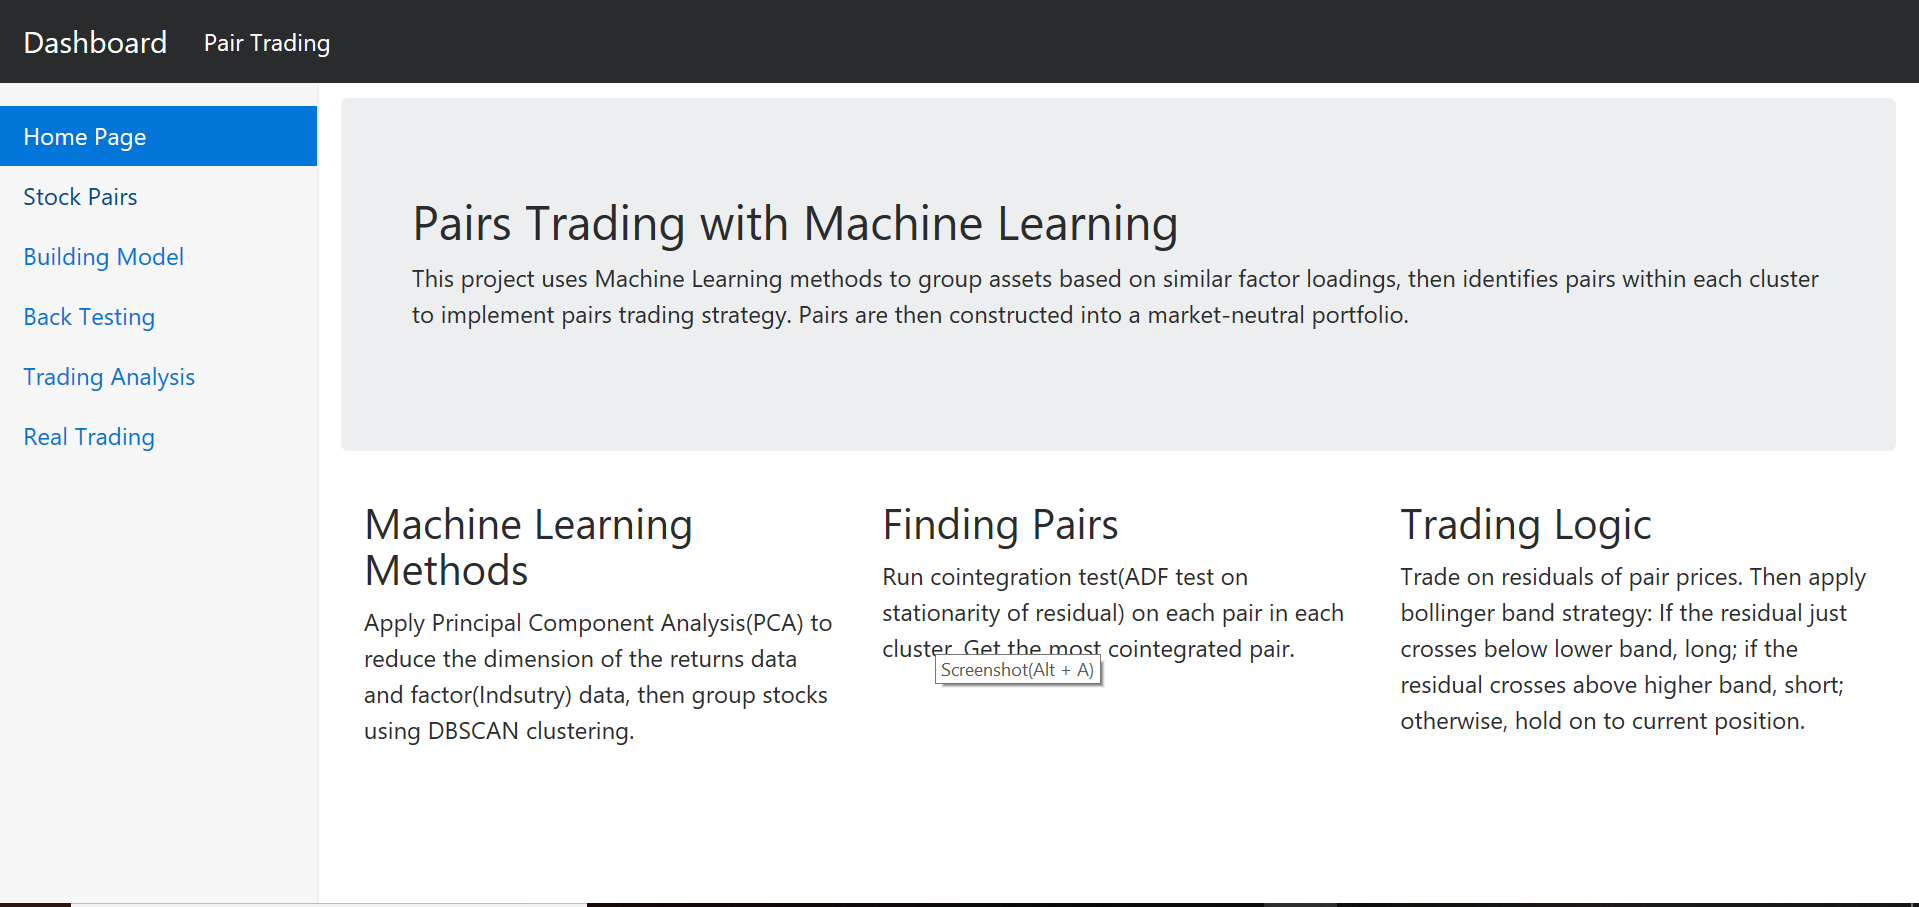
\includegraphics[scale=0.4]{performance_analysis/images/dashboard.png}
\caption{Dashboard Home Page}
\label{fig:dashboard}
\end{figure}

